\chapter{Introduction}
\section{Plastic Omnium}

Plastic Omnium est une entreprise fondée en 1946 par Pierre Burelle qui transforme et commercialise des matières plastiques, dont le chiffre d'affaires s'élève à plus de 5 milliards d'euros, dont 86\% réalisé à l'international. Cette compagnie française emploi plus de 22 000 collaborateurs qui travaillent dans 110 usines et 22 centres de recherche dans 29 pays.\\

L'entreprise est scindée en deux parties, Plastic Omnium Automobile et Plastic Omnium Environnement. Cette dernière est leader mondial de la conteneurisation des déchets, elle conçoit également des aires de jeux pour les collectivités.\\
Plastic Omnium Automobile regroupe Plastic Omnium Auto Exterior, leader mondial des pièces et modules de carrosserie et Inergy Automotive Systems, \no 1 mondial des systèmes à carburant. Avec des marques comme Peugeot, Renault, Toyota ou Porsche comme clients, les solutions de Plastic Omnium équipent plus d'une voiture sur cinq dans le monde. Les principaux objectifs sont de réduire le poids des véhicules et augmenter l'aérodynamisme afin de réduire les émissions, et équiper les véhicules hybrides et électriques. \\

Plastic Omnium dépense plus de 5\% de son CA en recherche et c'est pourquoi elle a crée en 2003 le centre de recherche $\Sigma$-Sigmatech à Sainte-Julie, où s'est déroulé mon stage.\\

\makebox[\textwidth][c]{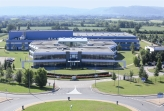
\includegraphics[scale=1.3]{img01_innovation}}

\section{Contexte du stage}

Le but de ce stage est d'explorer une méthode afin de réduire le temps de calcul lors de simulation des écoulements d'air sur la carrosserie d'une voiture, et plus précisément sur de pièces appelés ``spoilers'' ou ``vortex''. En effet, les turbulences à l'arrière du véhicule augmentent la consommation de carburant, et donc l'émission de $CO_2$. Ces pièces sont justement utilisées pour contrôler le flux d'air autour du véhicule et donc éviter les pertes d'énergies.\\

Cependant, la simulation de ces effets nécessite la résolution d'équations de Navier-Stokes avec un grand nombre d'inconnue, et est donc très coûteuse en temps de calcul. C'est pourquoi on s'intéresse à de nouvelles méthodes de résolutions de ces équations. Suivant les travaux du professeur Penel de l'université de Toulon, réalisé en collaboration avec le professeur Neustupa de la faculté de mathématiques de Pragues, on cherche à projeter la vitesse sur l'espace des fonctions propres de l'opérateur rotationnel, qui dépend uniquement de la géométrie. Ainsi, à chaque pas de temps, on aurait seulement à calculer les coefficients associés à cette projection. Cela conduirait à réduire le temps de calcul et donc de passer de une seconde de simulation à 10 secondes.\\

Cette idée a été étudiée par Benjamin Surowiek, qui a utilisé le logiciel FreeFem++ pour simulé des écoulements dans un cylindre. Cependant, la taille de la géométrie et la finesse de maillage demandée oblige à l'utilisation de logiciel de calcul permettant la résolution en parallèle des problèmes. Je dois donc utilisé Feel++ (Finite Element Embedded Library in C++, \cite{PRUDHOMME:2012:HAL-00662868:3,feelpp098:10046} ) pour implémenter le code nécessaire à la résolution d'un écoulement dans une géométrie simple, et comparer avec les différents résultats précédemment obtenus.

%%% Local Variables:
%%% TeX-master: "../report.tex"
%%% eval: (flyspell-mode 1)
%%% End:
